\documentclass[a4paper,fleqn]{cas-dc}

\usepackage[numbers]{natbib}
\usepackage{amsmath,amssymb,bm}
\usepackage{graphicx}
\graphicspath{{../figures/}}
\usepackage{booktabs}
\usepackage{xurl}
\usepackage{hyperref}
\hypersetup{hidelinks}
\usepackage{xcolor}
\usepackage{listings}
\usepackage{lineno}
\usepackage{float}
\usepackage{stfloats}
\usepackage{placeins}
\usepackage{enumitem}
\usepackage[protrusion=true,expansion=false]{microtype}
\usepackage{algorithm}
\usepackage{algpseudocode}
\usepackage{caption}
\usepackage{ragged2e}
\captionsetup[figure]{skip=4pt}

\graphicspath{{./}{figures/}}

\lstset{
  basicstyle=\ttfamily\small,
  frame=single,
  breaklines=true,
  columns=fullflexible,
  keepspaces=true
}

\begin{document}
\let\WriteBookmarks\relax
\renewcommand{\topfraction}{.95}
\renewcommand{\bottomfraction}{.9}
\renewcommand{\textfraction}{.05}
\renewcommand{\floatpagefraction}{.8}
\renewcommand{\dbltopfraction}{.95}
\renewcommand{\dblfloatpagefraction}{.75}
\setcounter{topnumber}{3}
\setcounter{bottomnumber}{2}
\setcounter{totalnumber}{5}
\setcounter{dbltopnumber}{3}

\shorttitle{DiracBench: Four-Method Relativistic Bound-State Benchmarks}
\shortauthors{Zalloum}

\title [mode = title]{DiracBench: A Reproducible Four-Method Framework for Relativistic Bound States with Scalar, Vector, and Tensor Interactions}

\author[1]{Othman H. Y. Zalloum}[orcid=0000-0001-7282-1332]
\cormark[1]
\ead{ozalloum@ppu.edu}
\affiliation[1]{organization={Palestine Polytechnic University},
            addressline={Department of Applied Mathematics and Physics},
            city={Hebron},
            country={Palestine}}
\cortext[1]{Corresponding author}

\begin{abstract}
We present DiracBench, a reproducible four-method framework for bound states of the spherical radial Dirac equation with scalar, vector, and radial tensor interactions. The implementation combines adaptive two-sided Runge--Kutta shooting, centered finite-difference matrix diagonalization, Chebyshev spectral collocation, and a dual-kinetic-balance (DKB) B-spline Galerkin discretization. Motivated by recent scalar--vector--tensor shooting calculations in coordinate space, but without reusing their fitted parameters or numerical results, we construct three independent dimensionless Woods--Saxon benchmark families and a controlled tensor-strength sweep. For the smooth benchmark P1, the four methods agree for the lowest states in the $\kappa=-1,1,-2$ channels with maximum cross-method spreads of $5.3\times10^{-6}$, $1.22\times10^{-5}$, and $1.12\times10^{-5}$, respectively. Across $U_0\in[-0.12,0.12]$, the maximum four-method spread remains below $8.4\times10^{-6}$. A domain-lock study shows the shooting energy stable to approximately $10^{-10}$ once $r_{\max}\ge20$ for P1. Phase-aligned common-grid comparisons give overlaps of $0.999990$ and $0.999514$ for finite differences and Chebyshev, respectively, relative to shooting. The centered finite-difference spectrum also exposes a grid-scale spurious state whose large component alternates sign at essentially every grid point, whereas the physical state has zero significant nodes. The DKB branch reaches few-$10^{-6}$ accuracy on the smooth benchmarks but exhibits non-monotonic basis refinement that remains a development target. The package contains the full numerical campaign, machine-readable CSV files, a dedicated error-analysis product, publication-quality figures, automated regression tests, a pseudocode-linked LaTeX manuscript, and a Jupyter notebook that is also compatible with Colab. These results establish an independent scalar--vector--tensor benchmark suite while retaining explicit diagnostics for unresolved discretization artifacts.
\end{abstract}

\begin{highlights}
\item Provides a reproducible four-method radial Dirac benchmark.
\item Tests shooting, finite differences, Chebyshev, and DKB B-splines.
\item Reports cross-method, residual, wavefunction, domain, and spurious-state diagnostics.
\item Includes portable scripts, tests, machine-readable data, and publication figures.
\end{highlights}

\begin{keywords}
Dirac equation \sep radial eigenvalue problem \sep kinetic balance \sep B splines \sep Chebyshev collocation \sep finite differences \sep reproducibility
\end{keywords}

\maketitle
\linenumbers
\RaggedRight

\section*{Program summary}
\noindent\textbf{Program title:} DiracBench: Scalar--Vector--Tensor Radial Dirac Benchmark Suite\\
\textbf{CPC library link to program files:} The complete source archive is available from the public repository and release link below; the CPC program-library record can be added after acceptance.\\
\textbf{Developer's repository link:} \url{https://github.com/ozalloum/diracbench}.\\
\textbf{Licensing provisions:} MIT.\\
\textbf{Programming language:} Python 3.\\
\textbf{External routines/libraries:} NumPy, SciPy, pandas, Matplotlib, and pytest.\\
\textbf{Nature of problem:} Reproducible computation of bound states of the spherical radial Dirac equation with scalar, vector, and radial tensor interactions, including the detection of discretization artifacts.\\
\textbf{Solution method:} Four independent numerical routes are implemented: adaptive two-sided shooting, centered finite-difference matrix diagonalization, Chebyshev collocation, and a dual-kinetic-balance B-spline Galerkin prototype.\\
\textbf{Restrictions:} The present campaign treats smooth dimensionless Woods--Saxon potentials and selected $\kappa$ channels; the centered finite-difference branch retains a documented grid-scale spurious mode, and the DKB refinement study is not uniformly monotone.\\
\textbf{Unusual features:} The release couples cross-method falsification, wavefunction overlap, residual and node diagnostics, domain locking, error-analysis tables, portable campaign execution, automated tests, and publication-quality figures.

\section{Introduction}
Reliable numerical solution of the Dirac equation requires more than obtaining apparently stable eigenvalues. First-order relativistic operators admit discretization artifacts that can masquerade as physical states, and finite basis representations require a controlled relationship between the large and small spinor components. Dual kinetic balance (DKB) was introduced to remove spurious states and improve convergence in finite-basis Dirac calculations \cite{Shabaev2004,Beloy2008}. Kinematically balanced B-spline approaches have subsequently been used successfully in relativistic eigenvalue problems \cite{Fillion2012,Fischer2009,Toffoli2003,Poschl1998}. More recently, Li \emph{et al.} showed explicitly that centered finite differences on a uniform radial grid can generate spurious states and proposed a staggered-grid scheme that suppresses the artifact \cite{Li2026,FillionGourdeau2012,Lewin2010}.

Complementary work has demonstrated the 3+1-dimensional free Dirac dynamics on a four-qubit superconducting platform, including signatures of Zitterbewegung and the Sauter--Schwinger effect \cite{Zhang2025}. That experimental program addresses dynamical emulation, whereas DiracBench targets the numerical validation of radial bound-state discretizations; the two perspectives motivate different but complementary reproducibility checks.

A recent coordinate-space solver by Kiessling \emph{et al.} applies two-sided Runge--Kutta shooting to spherical scalar, vector, and tensor Woods--Saxon potentials and discusses practical sensitivity to state identification and numerical implementation \cite{Kiessling2025,FillionGourdeau2012,Beerwerth2015,Lorin2022}. We use only these methodological ideas: no fitted parameters, energy tables, or wavefunctions from that work are reproduced here. Instead, all scalar--vector--tensor data below are generated from independent dimensionless benchmark sets defined specifically for DiracBench.

DiracBench is designed around cross-method falsification: a state is accepted only when independent discretizations converge to the same physical solution and pass residual, normalization, localization, node, and domain-size tests. CPC software studies have established useful precedents for radial Dirac solvers, B-spline programs, finite-element atomic calculations, partial-wave codes, and reusable relativistic software \cite{Certik2013,Zatsarinny2016,Tsoulos2019,Waide2020,Certik2024,Elsepa2021,Poskus2018,Bagci2022}. This manuscript documents the first reproducible prototype and, equally importantly, identifies the numerical branch that has not yet reached production quality.


\section{Radial Dirac formulation and common conventions}
We begin from the stationary Dirac equation
\begin{equation}
H\Psi(\mathbf r)=E\Psi(\mathbf r),
\end{equation}
with
\begin{equation}
H=
\boldsymbol{\alpha}\cdot\mathbf p
+\beta[m+S(r)]
+V(r)+H_T.
\end{equation}
In the standard representation,
\begin{equation}
\boldsymbol{\alpha}=
\begin{pmatrix}0&\boldsymbol{\sigma}\\ \boldsymbol{\sigma}&0\end{pmatrix},
\qquad
\beta=
\begin{pmatrix}I&0\\0&-I\end{pmatrix}.
\end{equation}
For spherical symmetry we use
\begin{equation}
\Psi_{\kappa m}(\mathbf r)=
\frac1r
\begin{pmatrix}
F(r)\Omega_{\kappa m}\\
iG(r)\Omega_{-\kappa m}
\end{pmatrix},
\end{equation}
together with
\begin{equation}
(\boldsymbol{\sigma}\!\cdot\!\hat{\mathbf r})\Omega_{\kappa m}
=-\Omega_{-\kappa m},
\qquad
(\boldsymbol{\sigma}\!\cdot\!\mathbf L+1)\Omega_{\kappa m}
=-\kappa\Omega_{\kappa m}.
\end{equation}
Using
\begin{equation}
\boldsymbol{\sigma}\cdot\mathbf p
=-i(\boldsymbol{\sigma}\cdot\hat{\mathbf r})
\left(
\frac{d}{dr}+\frac1r-\frac{\boldsymbol{\sigma}\cdot\mathbf L}{r}
\right),
\end{equation}
one obtains
\begin{align}
\boldsymbol{\sigma}\cdot\mathbf p
\left[\frac{F}{r}\Omega_{\kappa m}\right]
&=
\frac{i}{r}
\left(\frac{dF}{dr}+\frac{\kappa}{r}F\right)
\Omega_{-\kappa m},\\
\boldsymbol{\sigma}\cdot\mathbf p
\left[\frac{G}{r}\Omega_{-\kappa m}\right]
&=
\frac{i}{r}
\left(\frac{dG}{dr}-\frac{\kappa}{r}G\right)
\Omega_{\kappa m}.
\end{align}

For the radial tensor convention implemented in DiracBench,
\begin{equation}
K_\kappa(r)=\frac{\kappa}{r}-U(r).
\end{equation}
Introducing
\begin{equation}
\Sigma(r)=V(r)+S(r),
\qquad
\Delta(r)=V(r)-S(r),
\end{equation}
the radial equations are
\begin{align}
\left(\frac{d}{dr}+K_\kappa\right)F
&=[E+m-\Delta(r)]G,
\label{eq:radial1}\\
\left(\frac{d}{dr}-K_\kappa\right)G
&=-[E-m-\Sigma(r)]F.
\label{eq:radial2}
\end{align}
Equivalently,
\begin{align}
\frac{dF}{dr}
&=-K_\kappa F+[E+m-\Delta(r)]G,
\label{eq:firstF}\\
\frac{dG}{dr}
&=K_\kappa G-[E-m-\Sigma(r)]F.
\label{eq:firstG}
\end{align}
The common matrix form is
\begin{equation}
\begin{pmatrix}
m+\Sigma & -d/dr+K_\kappa\\
d/dr+K_\kappa & -m+\Delta
\end{pmatrix}
\binom{F}{G}
=
E\binom{F}{G}.
\label{eq:radialH}
\end{equation}

\subsection{Boundary behaviour}
For a point Coulomb potential $V=-Z\alpha/r$, the regular solution behaves as
\begin{equation}
F(r)\propto r^\gamma,
\qquad
\gamma=\sqrt{\kappa^2-(Z\alpha)^2},
\end{equation}
and the implemented convention gives
\begin{equation}
\frac{G}{F}=\frac{\gamma+\kappa}{Z\alpha}.
\end{equation}
For a bound state at large radius,
\begin{equation}
\lambda=\sqrt{m^2-E^2},
\qquad
F,G\propto e^{-\lambda r},
\qquad
\frac{G}{F}\sim-\frac{\lambda}{E+m}.
\end{equation}

\section{Numerical methods: integrated derivation, discretization, and pseudocode}
Each solver below is derived directly from the same radial operator. The derivation and algorithm are intentionally kept together so that every computational step can be traced to the underlying equations, following standard treatments of relativistic atomic structure and numerical differential equations \cite{Grant2007,Thaller1992,Hairer1993}.

\subsection{Adaptive two-sided shooting and Runge--Kutta integration}
With
\begin{equation}
\mathbf y=(F,G)^T,
\end{equation}
Eqs.~\eqref{eq:firstF}--\eqref{eq:firstG} become
\begin{equation}
\frac{d\mathbf y}{dr}=A(r;E)\mathbf y,
\end{equation}
where
\begin{equation}
A=
\begin{pmatrix}
-K_\kappa & E+m-\Delta\\
-[E-m-\Sigma] & K_\kappa
\end{pmatrix}.
\end{equation}
An outward solution and an inward solution represent the same eigenstate at
$r=r_m$ when they are linearly dependent. Hence
\begin{equation}
D(E)=
\det
\begin{pmatrix}
F_{\rm out}&F_{\rm in}\\
G_{\rm out}&G_{\rm in}
\end{pmatrix}_{r_m}
=
F_{\rm out}G_{\rm in}-G_{\rm out}F_{\rm in}=0.
\end{equation}
DiracBench finds the root of this secular function and then rescales and joins
the two integrations. The use of explicit bracketing, adaptive integration, and
domain refinement follows the convergence-oriented practice of open radial
Dirac solvers \cite{Certik2013,Hairer1993}.


\begin{algorithm}[t]
\caption{Adaptive two-sided shooting for one radial Dirac state}
\label{alg:shooting}
\begin{algorithmic}[1]
\Require $S,V,U,\kappa$, $[r_{\min},r_{\max}]$, energy bracket $[E_a,E_b]$
\Ensure Eigenvalue $E$ and normalized radial spinor $(F,G)$
\State Choose matching radius $r_m$
\For{each trial energy $E$ requested by the root finder}
\State Construct regular inner boundary data at $r_{\min}$
\State Integrate Eqs.~\eqref{eq:firstF}--\eqref{eq:firstG} outward to $r_m$
\State Construct exponentially decaying outer data at $r_{\max}$
\State Integrate inward from $r_{\max}$ to $r_m$
\State Evaluate $D(E)=F_{\rm out}G_{\rm in}-G_{\rm out}F_{\rm in}$
\EndFor
\State Root-find $D(E)=0$ inside the bracket
\State Reintegrate, rescale the inward branch, join, and normalize
\State \textbf{return} $E,F,G$
\end{algorithmic}
\end{algorithm}
\subsection{Finite-difference matrix diagonalization}
For
\begin{equation}
r_i=ih,\qquad h=\frac{r_{\max}}{N+1},
\end{equation}
the centered derivative is
\begin{equation}
f'(r_i)\approx\frac{f_{i+1}-f_{i-1}}{2h}.
\end{equation}
Thus
\begin{equation}
D_{i,i+1}=\frac1{2h},
\qquad
D_{i,i-1}=-\frac1{2h}.
\end{equation}
Defining
\begin{align}
A&=\mathrm{diag}[m+\Sigma(r_i)],\\
B&=\mathrm{diag}[-m+\Delta(r_i)],\\
K&=\mathrm{diag}[K_\kappa(r_i)],
\end{align}
gives
\begin{equation}
H_{\rm FD}=
\begin{pmatrix}
A&-D+K\\
D+K&B
\end{pmatrix}.
\end{equation}
The centered derivative has lattice symbol
\begin{equation}
\tilde D(k)=\frac{i\sin(kh)}{h},
\end{equation}
which vanishes at both $k=0$ and $k=\pi/h$. This extra zero explains the
fermion-doubling/spurious-mode risk and motivates a staggered-grid production
branch, consistent with the broader coordinate-space literature on suppressing
fermion doubling \cite{FillionGourdeau2012,Lewin2010}.


\begin{algorithm}[t]
\caption{Finite-difference eigensolver with spurious-state diagnostics}
\label{alg:fd}
\begin{algorithmic}[1]
\Require $S,V,U,\kappa,r_{\max},N$, target $E_t$
\Ensure Ranked physical-state candidates
\State Set $h=r_{\max}/(N+1)$; construct $r_i$ and centered derivative matrix $D$
\State Build diagonal matrices $A$, $B$, and $K$
\State Assemble the $2N\times2N$ block Hamiltonian from $A,B,D,$ and $K$
\State Compute several shift-invert eigenpairs near $E_t$
\For{each candidate $(E_j,F_j,G_j)$}
\State Normalize; compute residual, nodes, oscillation score, and tail weight
\State Check stability under grid and domain refinement
\EndFor
\State Flag grid-scale oscillatory or nonconvergent candidates
\State \textbf{return} ranked candidates
\end{algorithmic}
\end{algorithm}
\subsection{Chebyshev spectral collocation}
The Chebyshev--Lobatto nodes are
\begin{equation}
x_j=\cos\frac{j\pi}{N},
\qquad
j=0,\ldots,N,
\end{equation}
mapped by
\begin{equation}
r=\frac{r_{\max}}2(1-x).
\end{equation}
Therefore
\begin{equation}
\frac{d}{dr}=-\frac{2}{r_{\max}}\frac{d}{dx},
\qquad
D_r=-\frac{2}{r_{\max}}D_x.
\end{equation}
After eliminating endpoint degrees of freedom,
\begin{equation}
H_{\rm Ch}=
\begin{pmatrix}
A&-D_r+K\\
D_r+K&B
\end{pmatrix}.
\end{equation}
This global differentiation operator is independent of the local finite-
difference stencil and therefore provides a valuable cross-check. The
Chebyshev construction follows the standard spectral-collocation framework
\cite{Trefethen2000}.


\begin{algorithm}[t]
\caption{Chebyshev collocation solver}
\label{alg:cheb}
\begin{algorithmic}[1]
\Require $S,V,U,\kappa,r_{\max},N$, target $E_t$
\Ensure Collocation eigenpair and diagnostics
\State Form Lobatto nodes $x_j=\cos(j\pi/N)$ and map to $r_j$
\State Build $D_x$ and set $D_r=-2D_x/r_{\max}$
\State Remove endpoint degrees of freedom
\State Evaluate potentials and assemble $H_{\rm Ch}$
\State Diagonalize the dense collocation matrix
\State Reject eigenvalues with significant imaginary parts
\State Rank remaining states by target proximity, residual, and oscillation
\State \textbf{return} best physical candidate
\end{algorithmic}
\end{algorithm}
\subsection{Dual-kinetic-balance B-spline Galerkin discretization}
From Eq.~\eqref{eq:radial1},
\begin{equation}
G=
\frac{1}{E+m-\Delta}
\left(\frac{d}{dr}+K_\kappa\right)F.
\end{equation}
In the positive-energy nonrelativistic limit $E=m+\epsilon$ with
$|\epsilon|\ll m$ and weak potentials,
\begin{equation}
G\approx
\frac1{2m}
\left(\frac{d}{dr}+K_\kappa\right)F.
\label{eq:kb}
\end{equation}
A kinetically balanced basis therefore couples the small-component basis to
the differentiated large-component basis. This relation is the central
variational safeguard behind kinetic-balance and DKB constructions
\cite{Stanton1984,Kutzelnigg1984,Dyall1990,Beloy2008}. The DKB prototype uses
\begin{equation}
\begin{aligned}
u_i&=
\begin{pmatrix}
B_i\\
\frac{1}{2m}\left(\frac{d}{dr}+K_\kappa\right)B_i
\end{pmatrix},
\\[4pt]
v_i&=
\begin{pmatrix}
\frac{1}{2m}\left(-\frac{d}{dr}+K_\kappa\right)B_i\\
B_i
\end{pmatrix}.
\end{aligned}
\end{equation}
With
\begin{equation}
\Phi=\sum_i c_i u_i+\sum_i d_i v_i,
\end{equation}
Galerkin projection yields
\begin{equation}
HC=ESC,
\end{equation}
where
\begin{equation}
H_{ij}=\int\Phi_i^\dagger H_\kappa\Phi_j\,dr,
\qquad
S_{ij}=\int\Phi_i^\dagger\Phi_j\,dr.
\end{equation}


\begin{algorithm}[t]
\caption{Dual-kinetic-balance B-spline Galerkin solver}
\label{alg:dkb}
\begin{algorithmic}[1]
\Require $S,V,U,\kappa$, knots, spline degree $p$, basis size $N_B$
\Ensure Generalized eigenpairs and diagnostics
\State Construct endpoint-compatible B-splines $B_i$ and their derivatives
\For{each $B_i$}
\State Form the balanced spinors $u_i$ and $v_i$
\EndFor
\State Select radial quadrature and evaluate $H_{ij}$ and $S_{ij}$
\State Symmetrize roundoff in $H$ and $S$
\State Solve $HC=ESC$
\State Reconstruct and normalize candidate spinors
\State Evaluate residual, nodes, and basis/domain refinement
\State \textbf{return} physical candidates
\end{algorithmic}
\end{algorithm}
\section{Validation protocol and mathematical diagnostics}
\subsection{Residuals, normalization, and cross-method wavefunction agreement}
For a numerical spinor,
\begin{equation}
\mathbf R=(H_\kappa-E)\binom{F}{G},
\end{equation}
with
\begin{align}
R_F&=(m+\Sigma-E)F-\frac{dG}{dr}+K_\kappa G,\\
R_G&=\frac{dF}{dr}+K_\kappa F+(-m+\Delta-E)G.
\end{align}
The reported normalized residual is
\begin{equation}
\mathcal R=
\frac{
\left[\int(R_F^2+R_G^2)dr\right]^{1/2}}
{\left[\int(F^2+G^2)dr\right]^{1/2}}.
\end{equation}
After normalization,
\begin{equation}
\int(F^2+G^2)dr=1.
\end{equation}
Residual, overlap, and refinement checks are used together because variational
or Galerkin approximations of operators with a spectral gap can exhibit
spectral pollution even when isolated eigenvalues appear numerically stable
\cite{Grant1982,Lewin2010}.
For two independently computed real spinors, define
\begin{equation}
\mathcal O_{ij}=\int(F_iF_j+G_iG_j)\,dr,
\qquad
\sigma_{ij}=\mathrm{sgn}(\mathcal O_{ij}),
\end{equation}
and
\begin{equation}
\Delta\psi_{ij}=
\left[
\int
(F_i-\sigma_{ij}F_j)^2+
(G_i-\sigma_{ij}G_j)^2\,dr
\right]^{1/2}.
\end{equation}


\begin{algorithm}[t]
\caption{Cross-method validation of an identified physical state}
\label{alg:validate}
\begin{algorithmic}[1]
\Require Solutions from two or more independent solvers
\Ensure Energy, spinor, residual, and domain-agreement diagnostics
\State Interpolate all spinors to a common radial mesh and normalize
\For{each method pair $(i,j)$}
\State Compute $\Delta E_{ij}=|E_i-E_j|$
\State Compute signed overlap and choose the optimal global sign
\State Compute phase-aligned $\Delta\psi_{ij}$
\EndFor
\For{each method $i$}
\State Evaluate residual $\mathcal R_i$, nodes, oscillation, and tail localization
\State Repeat after increasing resolution and $r_{\max}$
\EndFor
\State Accept only states whose physical diagnostics converge consistently
\end{algorithmic}
\end{algorithm}
\subsection{Exact Dirac--Coulomb oracle and its derivation}
For
\begin{equation}
V=-\frac{Z\alpha}{r},
\qquad
S=U=0,
\end{equation}
define
\begin{equation}
\gamma=\sqrt{\kappa^2-(Z\alpha)^2},
\qquad
n_r=n-|\kappa|.
\end{equation}
The exact quantization condition is
\begin{equation}
\frac{Z\alpha E}{\sqrt{m^2-E^2}}
=n_r+\gamma.
\end{equation}
Squaring,
\begin{equation}
(Z\alpha)^2E^2=(n_r+\gamma)^2(m^2-E^2),
\end{equation}
so
\begin{equation}
E^2\left[(Z\alpha)^2+(n_r+\gamma)^2\right]
=m^2(n_r+\gamma)^2.
\end{equation}
Therefore
\begin{equation}
E_{n\kappa}
=
m\left[
1+\frac{(Z\alpha)^2}
{\left(n-|\kappa|+\sqrt{\kappa^2-(Z\alpha)^2}\right)^2}
\right]^{-1/2}.
\end{equation}
For $n=1$, $\kappa=-1$, $Z\alpha=0.2$, and $m=1$,
\begin{equation}
E=\sqrt{1-0.2^2}=0.9797958971132712.
\end{equation}
This analytic oracle follows the standard Dirac--Coulomb spectrum used in
relativistic atomic-structure calculations \cite{Thaller1992,Grant2007}.

\section{Original smooth scalar--vector--tensor benchmark design}
We define the independent Woods--Saxon family
\begin{equation} f(r;R,a)=\left[1+\exp\left(\frac{r-R}{a}\right)\right]^{-1}, \end{equation}
\begin{equation} S(r)=S_0f,\qquad V(r)=V_0f,\qquad U(r)=U_0f. \label{eq:wsbench}\end{equation}
All quantities in this campaign are dimensionless with $m=1$. The three parameter sets in Table~\ref{tab:paramsets} span a baseline well, a positive tensor perturbation, and a deeper/more diffuse well. They are not fits to any nucleus and are not copied from published numerical tables.
\begin{table}[t]\centering\caption{Original DiracBench smooth benchmark sets.}\label{tab:paramsets}\begin{tabular}{lrrrrr}\toprule Set & $S_0$ & $V_0$ & $U_0$ & $R$ & $a$\\\midrule P1&-0.60&0.20&0.00&5.0&0.60\\ P2&-0.60&0.20&0.08&5.0&0.60\\ P3&-0.70&0.25&-0.06&5.5&0.75\\\bottomrule\end{tabular}\end{table}
For each matrix method, the requested state is identified in the same $\kappa$ channel and tracked under refinement. Shift-invert targeting locates the relevant part of the spectrum but does not modify the independently assembled Hamiltonian.

\section{Four-method energy agreement}
\begin{table*}[t]\centering\caption{Four-method energies for P1 at $r_{\max}=25$. FD uses $N=900$, Chebyshev uses $N=120$, and DKB uses 46 B-splines of degree 5.}\label{tab:angular}\begin{tabular}{rrrrrr}\toprule $\kappa$ & Shooting & FD & Chebyshev & DKB B-spline & spread\\\midrule -1&0.7985749864&0.7985708513&0.7985749868&0.7985697115&$5.28\times10^{-6}$\\ 1&0.9725652688&0.9725550503&0.9725636160&0.9725672851&$1.22\times10^{-5}$\\ -2&0.9285358974&0.9285331465&0.9285359236&0.9285247109&$1.12\times10^{-5}$\\\bottomrule\end{tabular}\end{table*}
The largest spread is $1.22\times10^{-5}$. The three independent potential families give similarly small spreads:
\begin{table*}[t]\centering\caption{Lowest $\kappa=-1$ energies for the original parameter sets at $r_{\max}=30$.}\label{tab:sets}\begin{tabular}{lrrrrr}\toprule Set&Shooting&FD&Chebyshev&DKB B-spline&spread\\\midrule P1&0.7985749864&0.7985701621&0.7985749865&0.7985709189&$4.82\times10^{-6}$\\ P2&0.8258226101&0.8258186587&0.8258226101&0.8258190139&$3.95\times10^{-6}$\\ P3&0.7327349195&0.7327303606&0.7327349195&0.7327273352&$7.58\times10^{-6}$\\\bottomrule\end{tabular}\end{table*}
Figure~\ref{fig:agreement} visualizes both the energies and the absolute deviations from the independent shooting reference. The paired view makes the agreement scale visible without relying on rounded table entries.
\begin{figure*}[!t]
\centering
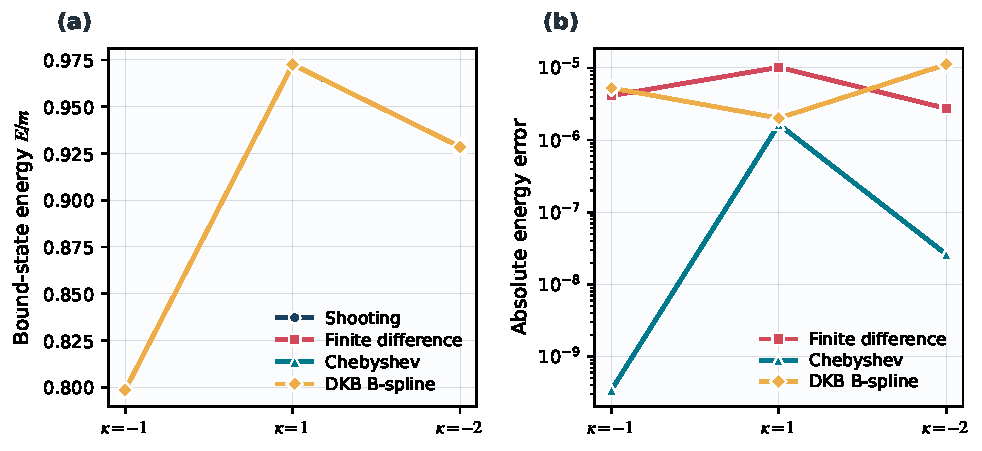
\includegraphics[width=.98\textwidth]{../figures/fig_method_agreement.pdf}
\caption{Baseline four-method agreement for the three angular channels. The left panel shows the identified energies; the right panel shows absolute deviations from two-sided shooting on a logarithmic scale.}
\label{fig:agreement}
\end{figure*}

\section{Error analysis and numerical reliability}
The release separates energy error, method-to-method spread, wavefunction agreement, domain truncation, and oscillatory-state diagnostics. For a matrix-method energy $E_i$ and the independently computed shooting energy $E_s$, we report $|E_i-E_s|$ and the relative error $|E_i-E_s|/|E_s|$. The cross-method spread is the maximum minus the minimum of the four energies for one identified state; it is a numerical-agreement measure rather than a statistical uncertainty.

For common-grid spinors, the global sign is chosen to make the overlap positive before computing the two-component $L^2$ difference. Domain error compares each shooting result with the largest tested domain, $r_{\max}=35$. Finally, the centered-FD alternation fraction records the proportion of adjacent large-component samples with opposite signs and is used together with node counts and cross-method disagreement to identify the grid-scale branch. All rows are written to \texttt{data/error\_analysis.csv}, with aggregate extrema in \texttt{data/error\_analysis\_summary.json}.
\begin{figure*}[!t]
\centering
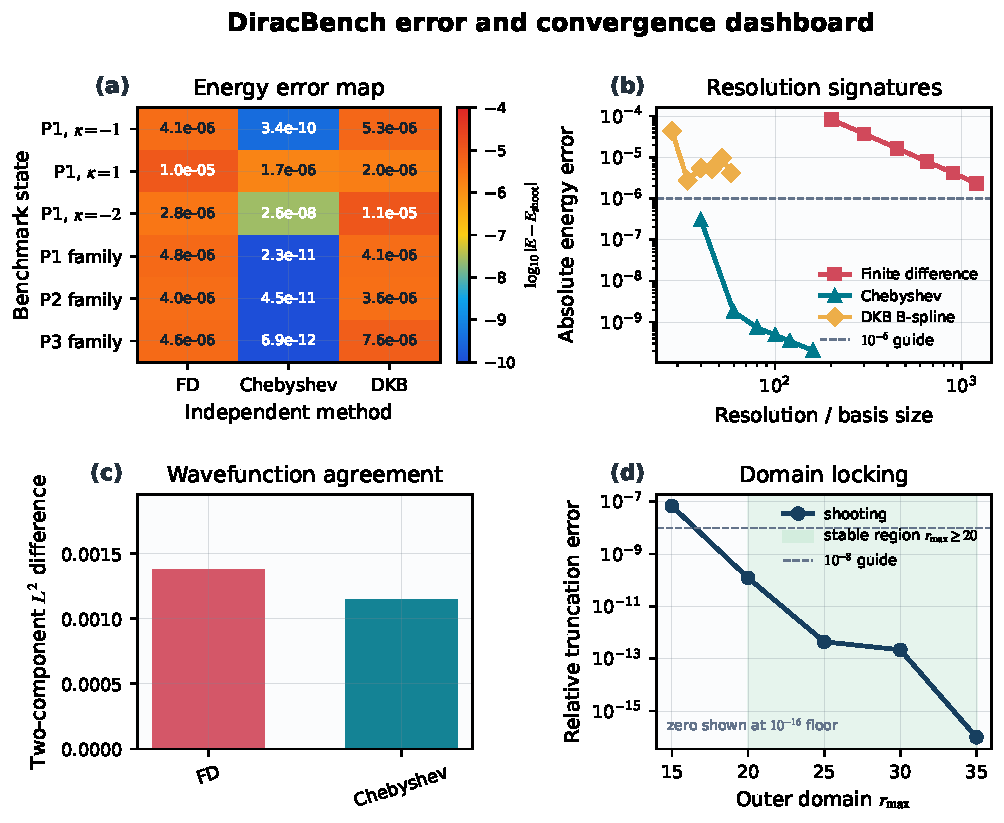
\includegraphics[width=.98\textwidth]{../figures/fig_error_analysis.pdf}
\caption{Error-analysis dashboard. (a) Annotated logarithmic energy-error map relative to shooting; (b) resolution signatures; (c) common-grid wavefunction differences, with FD and Chebyshev overlaps of $0.999990$ and $0.999514$, respectively; and (d) outer-domain locking. The diagnostics are complementary and are not interpreted as a single probabilistic error bar.}
\label{fig:errors}
\end{figure*}
\begin{figure*}[!t]
\centering
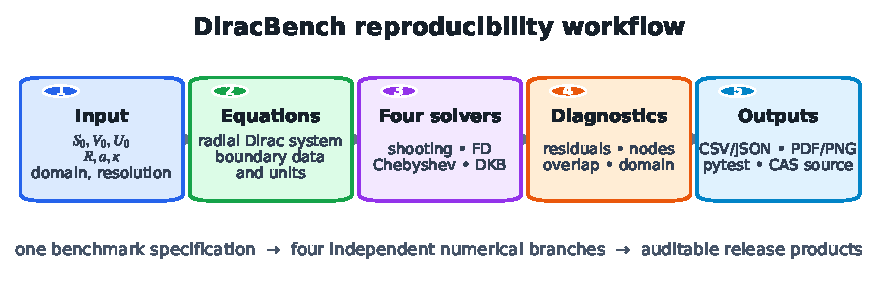
\includegraphics[width=.98\textwidth]{../figures/fig_diracbench_workflow.pdf}
\caption{Reproducible DiracBench workflow. A single benchmark specification is sent independently to the four numerical branches; the resulting energies and spinors are then checked by residual, normalization, node, overlap, and domain diagnostics before machine-readable data, vector figures, tests, and manuscript-ready outputs are written.}
\label{fig:workflow}
\end{figure*}

\section{Tensor-strength sweep}
The tensor interaction enters the radial operator through $K_\kappa(r)=\kappa/r-U(r)$ and changes the differential coupling between the large and small radial components without altering the scalar and vector Woods--Saxon profiles. It provides a controlled perturbation for testing whether the numerical methods follow the same bound-state branch. For P1, we hold $S_0=-0.60$, $V_0=0.20$, $R=5$, and $a=0.60$ fixed, and vary $U_0$ from $-0.12$ to $0.12$. The tracked lowest $\kappa=-1$ energy increases smoothly from $0.7578432$ to $0.8391539$. Shooting, finite differences, Chebyshev collocation, and DKB B-splines reproduce this trend. The maximum cross-method spread is $8.39\times10^{-6}$; this envelope measures numerical agreement, not statistical uncertainty. Its decrease toward positive $U_0$ records the observed conditioning of this branch, not a claim of superior accuracy. The complete sweep is retained in \texttt{data/tensor\_strength\_sweep.csv}, and the campaign driver and plotting script regenerate the values and figure independently.
\begin{figure*}[!t]
\centering
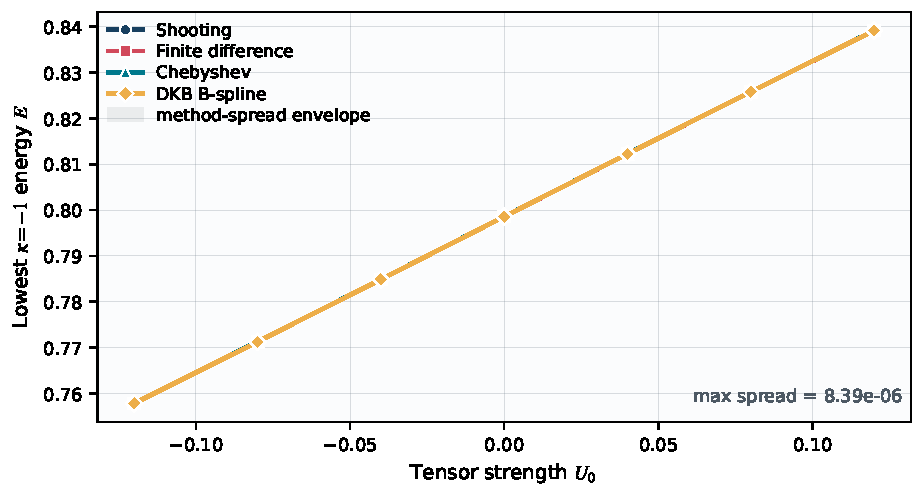
\includegraphics[width=.82\textwidth]{../figures/fig_tensor_sweep.pdf}
\caption{Tensor-strength response for P1. The shaded band is the four-method energy-spread envelope.}
\label{fig:tensor}
\end{figure*}
\FloatBarrier

\section{Domain-size and discretization refinement}
Figure~\ref{fig:rmax} varies $r_{\max}$ from 15 to 35 while maintaining approximately constant FD grid density and DKB basis density. The shooting energy changes from 0.7985749313 at $r_{\max}=15$ to 0.7985749863 at $r_{\max}=20$, and is then stable at approximately the $10^{-10}$ level. Chebyshev follows the same limit closely.
At fixed $r_{\max}=25$, the FD energy error decreases from $8.31\times10^{-5}$ at $N=200$ to $2.33\times10^{-6}$ at $N=1200$. Chebyshev falls below $2\times10^{-9}$ by $N=60$. The DKB calculation improves sharply between 28 and 34 basis functions but then fluctuates at the few-$10^{-6}$ level rather than converging monotonically; this plateau is retained explicitly.

\begin{figure*}[!t]
\centering
\begin{minipage}[t]{.48\textwidth}
\vspace{0pt}
\ExplSyntaxOn\dim_set:Nn \l_fig_width_dim {\linewidth}\ExplSyntaxOff
\centering
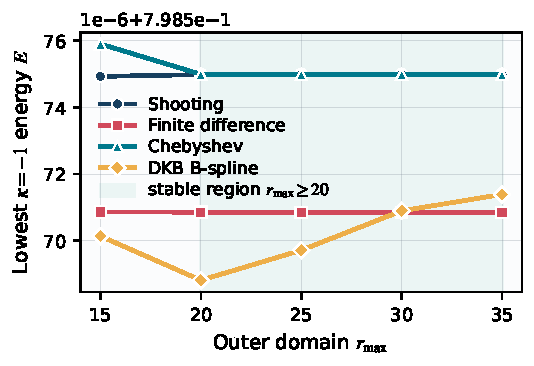
\includegraphics[width=\linewidth]{../figures/fig_rmax_independence.pdf}
\captionsetup{font=small}
\captionof{figure}{$r_{\max}$-independence test for the lowest P1 $\kappa=-1$ state. The highlighted region marks the domain range used for the stability claim.}
\label{fig:rmax}
\end{minipage}
\hfill
\begin{minipage}[t]{.48\textwidth}
\vspace{0pt}
\ExplSyntaxOn\dim_set:Nn \l_fig_width_dim {\linewidth}\ExplSyntaxOff
\centering
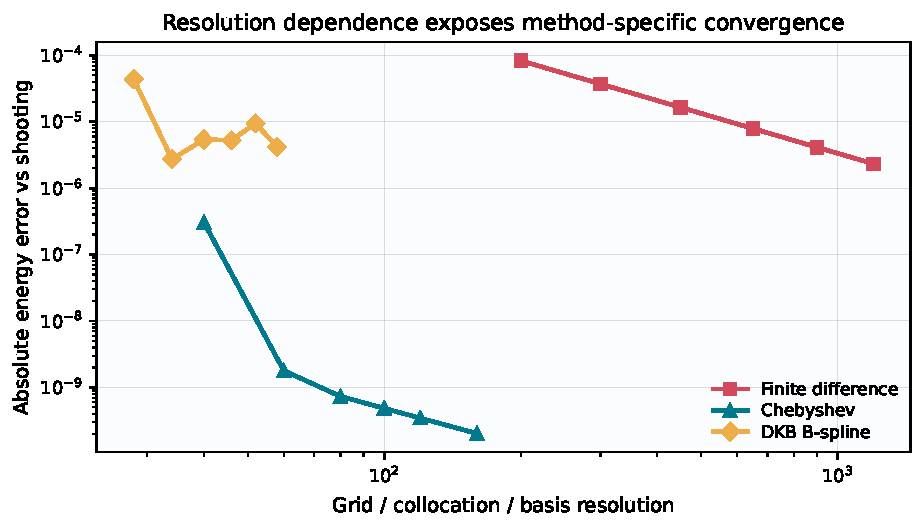
\includegraphics[width=\linewidth]{../figures/fig_resolution_convergence.pdf}
\captionsetup{font=small}
\captionof{figure}{Resolution study for P1, $\kappa=-1$, relative to the converged shooting energy. The finite-difference branch approaches the reference systematically, Chebyshev reaches the plotted floor rapidly, and the DKB values show the non-monotonic basis-refinement behavior discussed in the text.}
\label{fig:convnew}
\end{minipage}
\end{figure*}
\FloatBarrier

\begin{figure*}[!t]
\centering
\begin{minipage}[t]{.48\textwidth}
\vspace{0pt}
\ExplSyntaxOn\dim_set:Nn \l_fig_width_dim {\linewidth}\ExplSyntaxOff
\centering
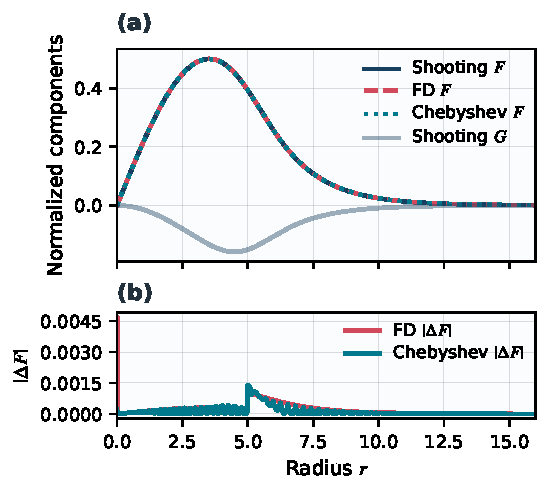
\includegraphics[width=\linewidth]{../figures/fig_wavefunction_comparison.pdf}
\captionsetup{font=small}
\captionof{figure}{Phase-aligned two-component wavefunction comparison for P1, $\kappa=-1$. The lower panel shows absolute differences in the large component relative to shooting.}
\label{fig:wave}
\end{minipage}
\hfill
\begin{minipage}[t]{.48\textwidth}
\vspace{0pt}
\ExplSyntaxOn\dim_set:Nn \l_fig_width_dim {\linewidth}\ExplSyntaxOff
\centering
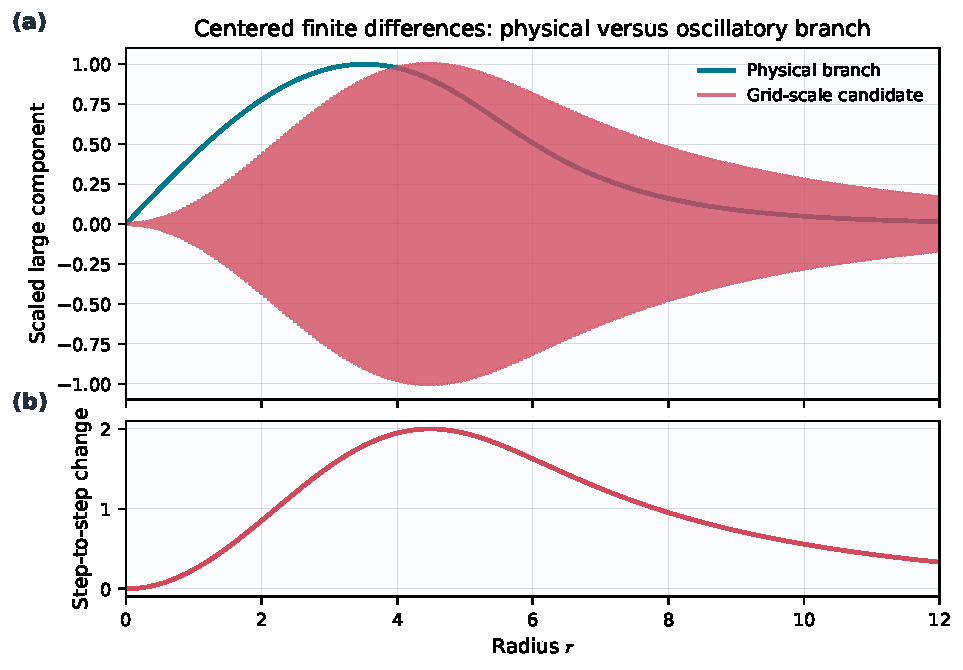
\includegraphics[width=\linewidth]{../figures/fig_fd_spurious_diagnostic.pdf}
\captionsetup{font=small}
\captionof{figure}{Centered-FD physical state and grid-scale oscillatory candidate for P1, $\kappa=-1$. The lower panel displays the step-to-step change that exposes the alternating branch.}
\label{fig:spur}
\end{minipage}
\end{figure*}

\section{Wavefunction agreement}
After common-grid renormalization and phase alignment, the FD--shooting overlap is 0.99998968 with two-component $L^2$ difference $1.38\times10^{-3}$, while the Chebyshev--shooting overlap is 0.99951424 with $L^2$ difference $1.15\times10^{-3}$. These are global two-component diagnostics; the energy agreement is substantially tighter than the pointwise wavefunction difference.

\section{Node and spurious-state diagnostics}
At $N=900$ in the P1 $\kappa=-1$ centered-FD calculation, the physical candidate at $E=0.7985708513$ has zero significant nodes and zero alternation fraction. A second positive candidate at $E=0.9725550503$ has 789 sign changes above a 1\% amplitude threshold and an alternation fraction of 1.0. Shooting and Chebyshev do not identify a corresponding physical bound state in this channel.

\section{Performance benchmark}
Median wall-clock times over three repetitions in the present Python environment are 0.0865 s for shooting, 0.0083 s for FD, 0.0316 s for Chebyshev, and 0.1440 s for DKB. These values are hardware- and implementation-dependent and are reported only as a reproducible baseline.

\begin{figure*}[!b]
\centering
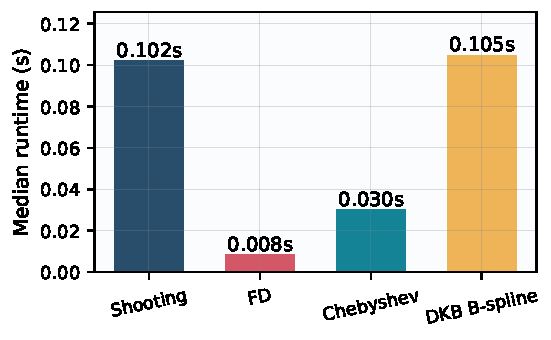
\includegraphics[width=.55\textwidth]{../figures/fig_performance.pdf}
\captionsetup{font=small}
\captionof{figure}{Median runtime baseline for one targeted P1 $\kappa=-1$ solve.}
\label{fig:performance}
\end{figure*}

\section{Additional spurious-state safeguards}
The explicit diagnostic above is supplemented by refinement checks and comparison with independent shooting and Chebyshev spectra. These tests are especially important because centered differences can generate spurious Dirac states \cite{Li2026,FillionGourdeau2012,Lewin2010}. A staggered-grid formulation, improved knot placement, and singular-potential validation are identified as next-stage work; the present release retains the centered scheme as a reproducible counterexample.

\section{Reproducibility and software}
The archive contains the reusable Python solver module, a portable campaign driver, a Jupyter notebook that is also compatible with Colab, CSV tables for every numerical sweep, a machine-readable error-analysis table, publication-quality PDF/PNG figures, automated regression tests, dependency metadata, an MIT license, and the present \LaTeX{} source.

The Python implementation uses the array, scientific-computing, plotting, and notebook ecosystems described by Harris \emph{et al.}, Virtanen \emph{et al.}, Hunter, and Kluyver \emph{et al.} \cite{Harris2020,Virtanen2020,Hunter2007,Kluyver2016}. The reproducibility record follows established recommendations for computational research and FAIR data stewardship \cite{Sandve2013,Wilkinson2016}, while the package-oriented release is consistent with CPC's open-source software tradition \cite{Scott2020}.

The command
\begin{verbatim}
python run_campaign.py \
  --output generated_campaign
\end{verbatim}
regenerates numerical outputs, error analysis, metadata, and figures without relying on a hard-coded path or deleting an existing output directory. All manuscript figures are regenerated from machine-readable outputs.

\begin{figure*}[!b]
\centering
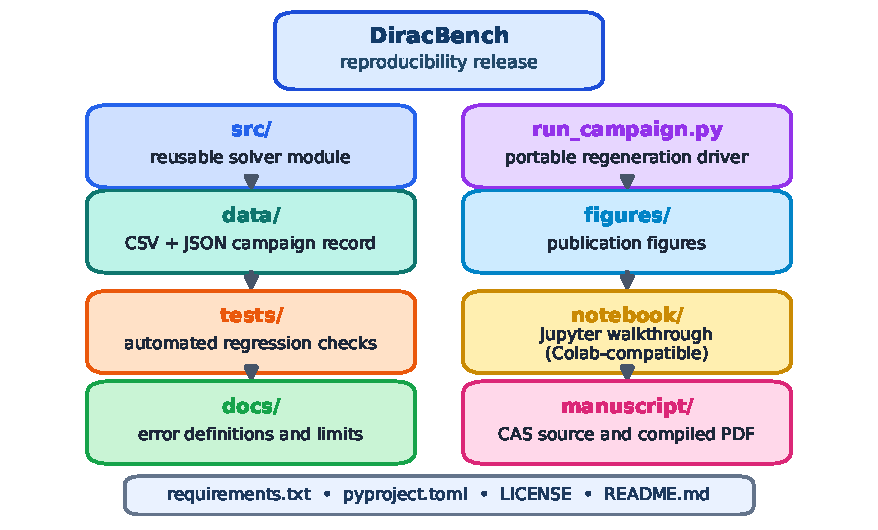
\includegraphics[width=.68\textwidth]{../figures/fig_diracbench_package_map.pdf}
\caption{Archive structure of the reproducibility release. Source code and the portable campaign driver generate CSV/JSON data and publication figures; tests, dependency metadata, the notebook, and the CAS manuscript remain visible as separately inspectable release components.}
\label{fig:package}
\end{figure*}
\FloatBarrier

\section{Limitations and next production stage}

The smooth-potential campaign establishes four-method agreement at the $10^{-5}$ scale or better for the tested states, but two limitations remain. First, the centered FD method still possesses the expected doubling artifact; its physical branch converges cleanly, while the oscillatory branch is retained as a reproducible diagnostic. Second, the DKB branch is accurate at the few-$10^{-6}$ level on the smooth benchmarks yet its basis-refinement curve is non-monotonic. The current release therefore reports conditioning and overlap diagnostics rather than presenting DKB as uniformly production-ready. A staggered-grid alternative, improved knot placement, and additional singular-potential validation are natural next steps. The singular point-Coulomb DKB benchmark remains separate and is not used to support the smooth-potential four-method claim.
% Place every pending figure before the concluding section.
\FloatBarrier
\section{Conclusions}

DiracBench provides an original numerical scalar--vector--tensor campaign spanning three smooth Woods--Saxon parameter sets, three angular channels, tensor-strength and convergence studies, wavefunction comparisons, node diagnostics, and runtime measurements. For the principal tests, all four methods identify the same bound states with cross-method energy spreads below $1.3\times10^{-5}$; the tensor sweep remains below $8.4\times10^{-6}$. Shooting and Chebyshev show near-identical energies, FD converges systematically, and DKB reaches few-$10^{-6}$ accuracy while retaining a reported non-monotonic basis plateau. The grid-scale oscillatory FD state further demonstrates the value of combined node and cross-method diagnostics.

\section*{Data and code availability}
All source code, dependency metadata, the MIT license, automated tests, the Jupyter notebook (Colab-compatible), CSV outputs, error-analysis products, publication figures, and figure-generation scripts used for the scalar--vector--tensor campaign are included in the accompanying reproducibility archive.

The source repository is publicly available at
\url{https://github.com/ozalloum/diracbench}.\\
The exact reproducibility package is archived in the public release
\url{https://github.com/ozalloum/diracbench/releases/tag/1.0.0}.

\section*{Declarations}
\noindent\textbf{Funding:} This research did not receive any specific grant from funding agencies in the public, commercial, or not-for-profit sectors.\par\smallskip
\noindent\textbf{Acknowledgements:} The author acknowledges Palestine Polytechnic University for its support.\par\smallskip
\noindent\textbf{Competing interests:} The author declares that there are no known competing financial interests or personal relationships that could have appeared to influence the work reported in this paper.\par\smallskip
\noindent\textbf{Data and code:} The data and source-code availability statement above describes the public repository and reproducibility release.\par\smallskip
\noindent\textbf{Generative-AI assistance:} During manuscript preparation, the author used ChatGPT for language editing, clarity improvement, and manuscript-formatting support. The author reviewed and edited the output and takes full responsibility for the published content; numerical data, figures, and scientific conclusions were produced from the released computational workflow.
\renewcommand{\bibsection}{}
\section*{References}

\begin{thebibliography}{00}

\bibitem{Shabaev2004} V. M. Shabaev, I. I. Tupitsyn, V. A. Yerokhin, G. Plunien, G. Soff, Dual Kinetic Balance Approach to Basis-Set Expansions for the Dirac Equation, Phys. Rev. Lett. 93 (2004) 130405, \url{https://doi.org/10.1103/PhysRevLett.93.130405}.

\bibitem{Li2026} L. Li, H. Shen, J. Hu, Y. Zhang, Resolving the spurious-state problem in the Dirac equation by using the staggered-grid method, Phys. Rev. C 113 (2026) 034315, \url{https://doi.org/10.1103/n376-m3nf}.

\bibitem{Fillion2012} F. Fillion-Gourdeau, E. Lorin, A. D. Bandrauk, Numerical solution of the time-independent Dirac equation for diatomic molecules: B splines without spurious states, Phys. Rev. A 85 (2012) 022506, \url{https://doi.org/10.1103/PhysRevA.85.022506}.

\bibitem{Fischer2009} C. Froese Fischer, O. Zatsarinny, A B-spline Galerkin method for the Dirac equation, Comput. Phys. Commun. 180 (2009) 879--886, \url{https://doi.org/10.1016/j.cpc.2008.12.010}.

\bibitem{Kiessling2025} A. W. Kiessling, D. Karlsson, Y. Zhao, M. Bettencourt Amaro, C. Qi, Numerical solution of the Dirac equation with scalar, vector, and tensor potentials, Nucl. Sci. Tech. 36 (2025) 234, \url{https://doi.org/10.1007/s41365-025-01810-4}.

\bibitem{Zhang2025} Y. Zhang, J. Xu, Z. Ma, W. Zheng, D. Lan, X. Tan, Y. Yu, Experimental simulation of Dirac equation in superconducting qubits, Communications Physics 8 (2025) 248, \url{https://doi.org/10.1038/s42005-025-02112-2}.

\bibitem{Toffoli2003} D. Toffoli, P. Decleva, Least squares B-spline solutions of the radial Dirac equation in the continuum, Comput. Phys. Commun. 152 (2003) 151--164, \url{https://doi.org/10.1016/S0010-4655(02)00820-2}.

\bibitem{Poschl1998} W. P\"oschl, B-spline finite elements and their efficiency in solving relativistic mean field equations, Comput. Phys. Commun. 112 (1998) 42--66, \url{https://doi.org/10.1016/S0010-4655(98)00003-4}.

\bibitem{Beloy2008} K. Beloy, A. Derevianko, Application of the dual-kinetic-balance sets in the relativistic many-body problem of atomic structure, Comput. Phys. Commun. 179 (2008) 310--319, \url{https://doi.org/10.1016/j.cpc.2008.03.004}.

\bibitem{FillionGourdeau2012} F. Fillion-Gourdeau, E. Lorin, A. D. Bandrauk, Numerical solution of the time-dependent Dirac equation in coordinate space without fermion-doubling, Comput. Phys. Commun. 183 (2012) 1403--1415, \url{https://doi.org/10.1016/j.cpc.2012.02.012}.

\bibitem{Certik2013} O. Certik, J. E. Pask, J. Vackar, dftatom: A robust and general Schr\"odinger and Dirac solver for atomic structure calculations, Comput. Phys. Commun. 184 (2013) 1777--1791, \url{https://doi.org/10.1016/j.cpc.2013.02.014}.

\bibitem{Beerwerth2015} R. Beerwerth, H. Bauke, Krylov subspace methods for the Dirac equation, Comput. Phys. Commun. 188 (2015) 189--197, \url{https://doi.org/10.1016/j.cpc.2014.11.008}.

\bibitem{Zatsarinny2016} O. Zatsarinny, C. Froese Fischer, DBSR\_HF: A B-spline Dirac--Hartree--Fock program, Comput. Phys. Commun. 202 (2016) 287--303, \url{https://doi.org/10.1016/j.cpc.2015.12.023}.

\bibitem{Tsoulos2019} I. G. Tsoulos, O. T. Kosmas, V. N. Stavrou, DiracSolver: A tool for solving the Dirac equation, Comput. Phys. Commun. 236 (2019) 237--243, \url{https://doi.org/10.1016/j.cpc.2018.10.010}.

\bibitem{Waide2020} D. T. Waide, D. G. Green, G. F. Gribakin, BSHF: A program to solve the Hartree--Fock equations for arbitrary central potentials using a B-spline basis, Comput. Phys. Commun. 250 (2020) 107112, \url{https://doi.org/10.1016/j.cpc.2019.107112}.

\bibitem{Bagci2022} A. Bagci, JRAF: A Julia package for computation of relativistic molecular auxiliary functions, Comput. Phys. Commun. 273 (2022) 108276, \url{https://doi.org/10.1016/j.cpc.2021.108276}.

\bibitem{Lorin2022} E. Lorin, X. Yang, Time-dependent Dirac equation with physics-informed neural networks: Computation and properties, Comput. Phys. Commun. 280 (2022) 108474, \url{https://doi.org/10.1016/j.cpc.2022.108474}.

\bibitem{Certik2024} O. Certik, J. E. Pask, I. Fernando, R. Goswami, N. Sukumar, L. A. Collins, G. Manzini, J. Vackar, High-order finite element method for atomic structure calculations, Comput. Phys. Commun. 297 (2024) 109051, \url{https://doi.org/10.1016/j.cpc.2023.109051}.

\bibitem{Poskus2018} A. Poskus, BREMS: A program for calculating spectra and angular distributions of bremsstrahlung at electron energies less than 3 MeV, Comput. Phys. Commun. 232 (2018) 237--255, \url{https://doi.org/10.1016/j.cpc.2018.04.030}.

\bibitem{Scott2020} N. S. Scott, A. Hibbert, J. Ballantyne, S. Fritzsche, A. L. Hazel, D. P. Landau, D. W. Walker, Z. Was, CPC's 50th Anniversary: Celebrating 50 years of open-source software in computational physics, Comput. Phys. Commun. 252 (2020) 107269, \url{https://doi.org/10.1016/j.cpc.2020.107269}.

\bibitem{Elsepa2021} F. Salvat, A. Jablonski, C. J. Powell, elsepa---Dirac partial-wave calculation of elastic scattering of electrons and positrons by atoms, positive ions and molecules (New Version Announcement), Comput. Phys. Commun. 261 (2021) 107704, \url{https://doi.org/10.1016/j.cpc.2020.107704}.

\bibitem{Stanton1984} R. E. Stanton, S. Havriliak, Kinetic balance: A partial solution to the problem of variational safety in Dirac calculations, J. Chem. Phys. 81 (1984) 1910--1918, \url{https://doi.org/10.1063/1.447865}.

\bibitem{Grant1982} I. P. Grant, Conditions for convergence of variational solutions of Dirac's equation in a finite basis, Phys. Rev. A 25 (1982) 1230--1232, \url{https://doi.org/10.1103/PhysRevA.25.1230}.

\bibitem{Kutzelnigg1984} W. Kutzelnigg, Basis set expansion of the Dirac operator without variational collapse, Int. J. Quantum Chem. 25 (1984) 107--129, \url{https://doi.org/10.1002/qua.560250112}.

\bibitem{Dyall1990} K. G. Dyall, K. F\ae gri, Jr., Kinetic balance and variational bounds failure in the solution of the Dirac equation in a finite Gaussian basis set, Chem. Phys. Lett. 174 (1990) 25--32, \url{https://doi.org/10.1016/0009-2614(90)85321-3}.

\bibitem{Lewin2010} M. Lewin, E. S\'er\'e, Spectral pollution and how to avoid it, Proc. Lond. Math. Soc. 100 (2010) 864--900, \url{https://doi.org/10.1112/plms/pdp046}.

\bibitem{Thaller1992} B. Thaller, The Dirac Equation, Springer, Berlin, 1992, \url{https://doi.org/10.1007/978-3-662-02753-0}.

\bibitem{Grant2007} I. P. Grant, Relativistic Quantum Theory of Atoms and Molecules: Theory and Computation, Springer, New York, 2007, \url{https://doi.org/10.1007/978-0-387-35069-1}.

\bibitem{Hairer1993} E. Hairer, S. P. N\"orsett, G. Wanner, Solving Ordinary Differential Equations I: Nonstiff Problems, 2nd revised ed., Springer, Berlin, 1993, \url{https://doi.org/10.1007/978-3-540-78862-1}.

\bibitem{Trefethen2000} L. N. Trefethen, Spectral Methods in MATLAB, SIAM, Philadelphia, 2000, \url{https://doi.org/10.1137/1.9780898719598}.

\bibitem{Harris2020} C. R. Harris et al., Array programming with NumPy, Nature 585 (2020) 357--362, \url{https://doi.org/10.1038/s41586-020-2649-2}.

\bibitem{Virtanen2020} P. Virtanen et al., SciPy 1.0: Fundamental Algorithms for Scientific Computing in Python, Nature Methods 17 (2020) 261--272, \url{https://doi.org/10.1038/s41592-019-0686-2}.

\bibitem{Hunter2007} J. D. Hunter, Matplotlib: A 2D graphics environment, Comput. Sci. Eng. 9 (2007) 90--95, \url{https://doi.org/10.1109/MCSE.2007.55}.

\bibitem{Sandve2013} G. K. Sandve, A. Nekrutenko, J. Taylor, E. Hovig, Ten Simple Rules for Reproducible Computational Research, PLoS Comput. Biol. 9 (2013) e1003285, \url{https://doi.org/10.1371/journal.pcbi.1003285}.

\bibitem{Wilkinson2016} M. D. Wilkinson et al., The FAIR Guiding Principles for scientific data management and stewardship, Sci. Data 3 (2016) 160018, \url{https://doi.org/10.1038/sdata.2016.18}.

\bibitem{Kluyver2016} T. Kluyver, B. Ragan-Kelley, F. P\'erez, B. Granger, M. Bussonnier, J. Frederic, K. Kelley, J. Hamrick, J. Grout, S. Corlay, P. Ivanov, D. Avila, S. Abdalla, C. Willing, Jupyter Notebooks---a publishing format for reproducible computational workflows, in: F. Loizides, B. Schmidt (Eds.), Positioning and Power in Academic Publishing: Players, Agents and Agendas, IOS Press, Amsterdam, 2016, pp. 87--90, \url{https://doi.org/10.3233/978-1-61499-649-1-87}.

\end{thebibliography}

\end{document} 
